\documentclass{article}

\usepackage{graphicx}
\usepackage{tikz}
\usepackage{tikzsymbols}
\usetikzlibrary{calc,patterns,shapes.geometric}
\pagestyle{empty}
\usepackage[margin=0pt]{geometry}
\geometry{papersize={14in,12in}}

\def\centerarc[#1](#2)(#3:#4:#5){\draw[#1] ($(#2)+({#5*cos(#3)},{#5*sin(#3)})$) arc (#3:#4:#5);}

\begin{document}
	\begin{figure}
		\centering
		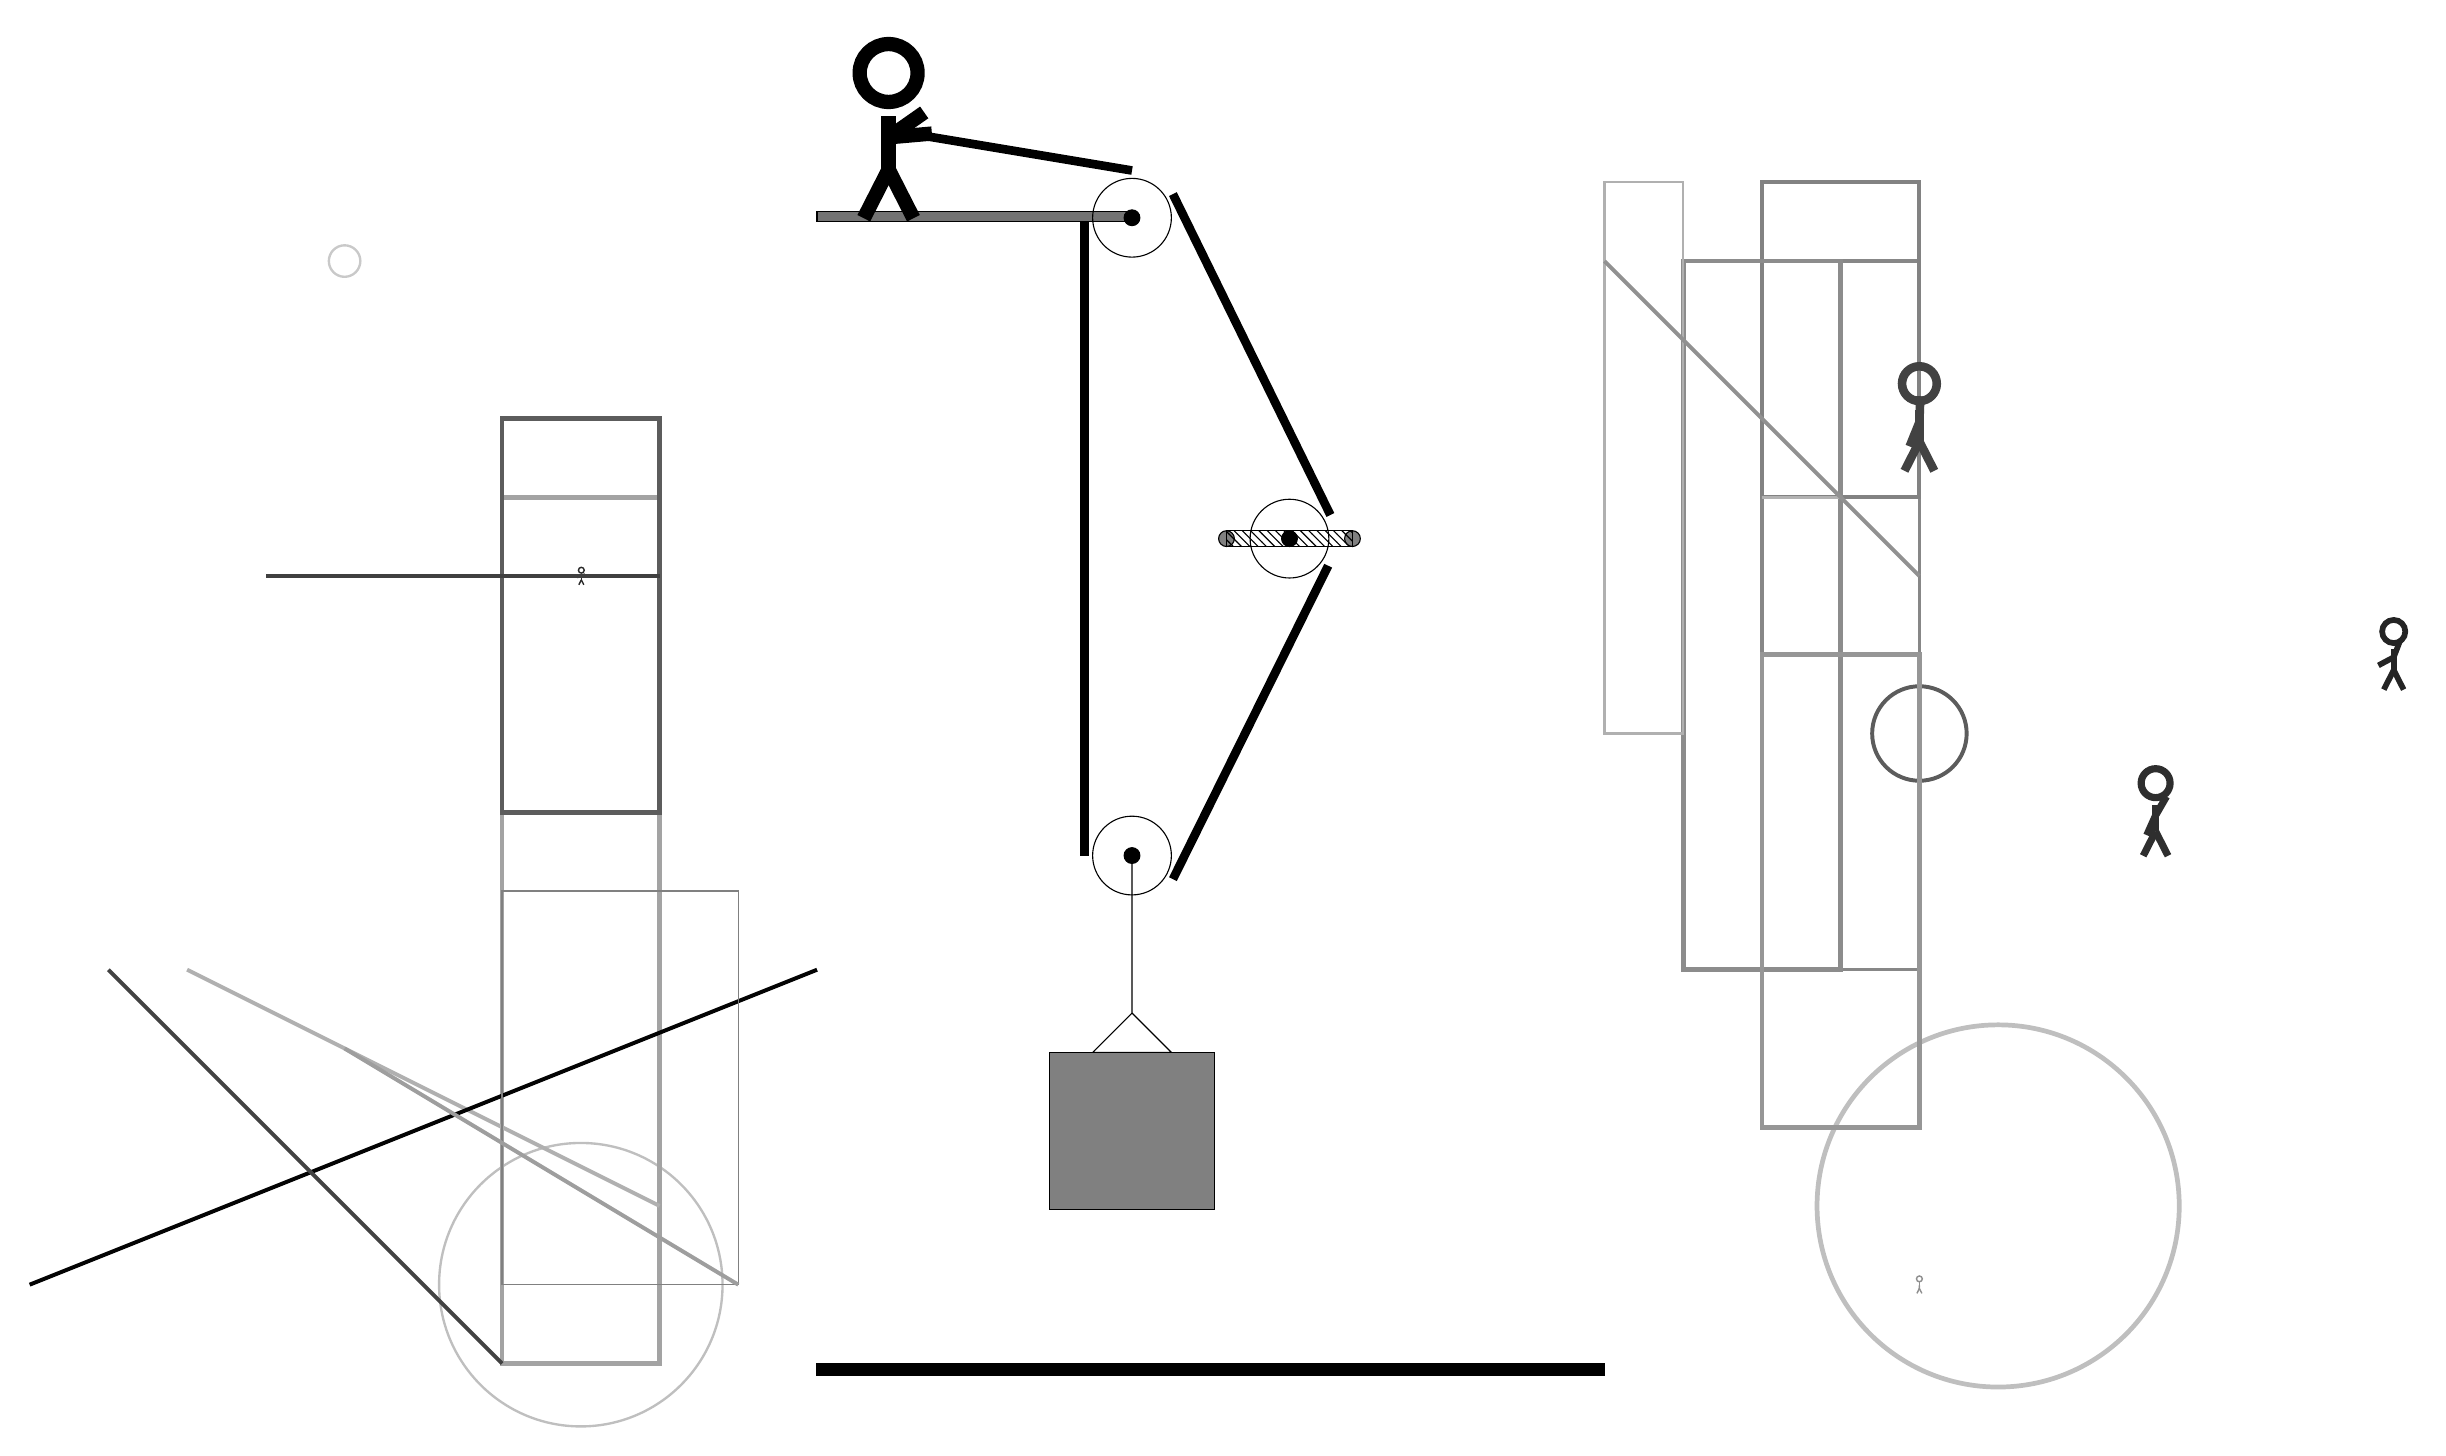
\begin{tikzpicture}
			%%%%% START %%%%%
			
			\draw[fill=black!55] (-2, 11.5) rectangle (2, 11.625);
			
			\draw (2, 3.45) circle (0.5);
			\draw[fill=black] (2, 3.45) circle (0.1);
			
			\draw (2, 11.55) circle (0.5);
			\draw[fill=black] (2, 11.55) circle (0.1);
			
			\draw[fill=white](4, 7.475) circle (0.5);
			\draw[fill=black] (4, 7.475) circle (0.1);
			\draw[fill=black!50] (3.2, 7.475) circle (0.1);
			\draw[fill=black!50] (4.8, 7.475) circle (0.1);
			\draw[pattern=north west lines, pattern color=black] (3.2, 7.575) rectangle (4.8, 7.375);
			
			\draw (2, 3.45) -- (2, 1.45) -- (1.5, 0.95) -- (2.5, 0.95) -- (2, 1.45);
			\draw[fill=black!50] (0.95, 0.95) rectangle (3.05, -1.05);
			
			\draw[line width=1.1mm] (1.4, 11.5) -- (1.4, 3.45);
			\centerarc[line width=1.1mm](2, 3.45)(180:330:0.6);
			\draw[line width=1.1mm](2.5196, 3.15) -- (4.4915, 7.1308);
			\centerarc[line width=1.1mm](4, 7.475)(390:325:0.6);
			\draw[line width=1.1mm](4.5196, 7.775) -- (2.5196, 11.85);
			\centerarc[line width=1.1mm](2, 11.55)(30:90:0.6);
			\draw[line width=1.1mm](2, 12.15) -- (-1, 12.65);
			
			\node[line width=0.7mm, color=black!84] at (-5, 7) {\Strichmaxerl[1][12][42]};
			
			\draw [line width=0.3mm, color=black!25](-5, -2) circle (1.8);
			\node[line width=0.4mm, color=black!86] at (18, 6) {\Strichmaxerl[4][28][69]};
			\draw[line width=0.4mm, color=black!47] (10, 2) rectangle (12, 11);
			\draw[line width=0.5mm, color=black!49] (10, 8) rectangle (12, 12);
			
			\draw[line width=0.6mm, color=black!45] (9, 11) rectangle (11, 2);
			\draw[line width=0.6mm, color=black!36] (-4, 8) rectangle (-6, -3);
			\draw [line width=0.6mm, color=black!25](13, -1) circle (2.3);
			\draw [line width=0.3mm, color=black!21](-8, 11) circle (0.2);
			
			\draw[line width=0.6mm, color=black!64] (-4, 4) rectangle (-6, 9);
			\draw[line width=0.5mm, color=black!31](-4, -1) -- (-10, 2);
			\draw[line width=0.5mm, color=black!99](-2, 2) -- (-12, -2);
			\draw[line width=0.5mm, color=black!74](-6, -3) -- (-11, 2);
			
			\node[line width=0.2mm, color=black!74] at (12, 9) {\Strichmaxerl[6][68][88]};
			\draw[line width=0.4mm, color=black!30] (10, 8) rectangle (11, 8);
			\draw[line width=0.2mm, color=black!50] (-3, -2) rectangle (-6, 3);
			\draw[line width=0.5mm, color=black!38](-3, -2) -- (-8, 1);
			\draw[line width=0.3mm, color=black!31] (8, 12) rectangle (9, 5);
			\draw[line width=0.5mm, color=black!75](-4, 7) -- (-9, 7);
			\draw[line width=0.5mm, color=black!43](12, 7) -- (8, 11);
			\draw [line width=0.5mm, color=black!64](12, 5) circle (0.6);
			\draw[line width=0.6mm, color=black!41] (10, 6) rectangle (12, 0);
			\node[line width=0.5mm, color=black!44] at (12, -2) {\Strichmaxerl[1][87][90]};
			\node[line width=0.4mm, color=black!82] at (15, 4) {\Strichmaxerl[5][66][60]};
			
			\node at (-1, 12.65) {\Strichmaxerl[10][-175][35]};
			
			\draw[fill=black] (-2, -3) rectangle (8, -3.15);
			
			%%%%% END %%%%%
		\end{tikzpicture}
	\end{figure}	
\end{document}